\documentclass[10pt,a4paper]{article}
\usepackage[margin=22mm]{geometry}
\usepackage[T1]{fontenc}
\usepackage{lmodern,amsmath,amssymb,booktabs,graphicx,tikz,hyperref,fvextra}
\usetikzlibrary{arrows.meta,positioning,calc,decorations.pathmorphing}
\definecolor{ink}{RGB}{20,53,78}
\hypersetup{colorlinks=true,urlcolor=ink,linkcolor=ink}
\setlength{\parindent}{0pt}
\setlength{\parskip}{5pt}
\emergencystretch=3em

\title{\color{ink}Lead-lag design for a normalized camera axis}
\author{}
\date{Original learning collection -- November 2026}
\begin{document}
\begin{center}{\LARGE\color{ink}Lead-lag design for a normalized camera axis}\\[5pt]{\small Original learning collection -- November 2026}\end{center}

\textbf{Evidence note.} Original teaching scenario. Numerical parameters are deliberately chosen for learning. All generated data and curves are synthetic; no physical measurement is asserted.
\section{Design brief}
For $G(s)=1/[s(s+1)]$, design lead compensation with crossover $\omega_c=3\,\mathrm{rad/s}$ and target phase margin $55^\circ$, centering maximum lead at crossover. Add lag zero $0.03\,\mathrm{rad/s}$ and pole $0.006\,\mathrm{rad/s}$, then renormalize gain at $\omega_c$. Compare final phase margins, velocity constants $K_v$, ramp errors and reference responses.
\section{Physical system}
\begin{center}\resizebox{\ifdim\width>.98\linewidth.98\linewidth\else\width\fi}{!}{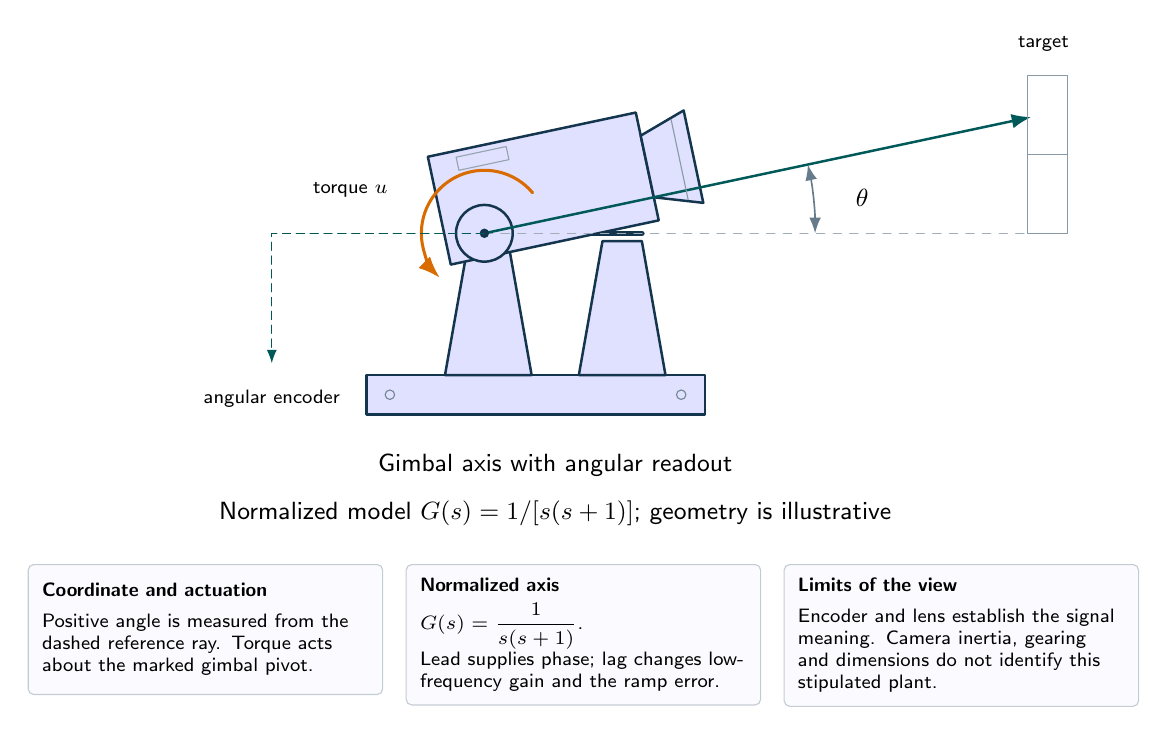
\begin{tikzpicture}[
font=\sffamily\small,>=Latex,line cap=round,line join=round,
wall/.style={draw=ink,line width=1.2pt,fill=blue!5},
water/.style={fill=cyan!25,draw=none},
metal/.style={draw=ink,fill=blue!12,line width=.9pt},
flow/.style={->,draw=blue!65!black,line width=1.2pt},
heat/.style={->,draw=orange!85!black,line width=1.1pt},
measure/.style={->,draw=teal!70!black,line width=.9pt},
dim/.style={<->,draw=ink!65,line width=.6pt},
spring/.style={draw=ink,decorate,decoration={coil,aspect=.5,segment length=4pt,amplitude=3pt}},
wire/.style={draw=ink,line width=1pt},
lab/.style={align=center,font=\sffamily\small},
smalllab/.style={align=center,font=\sffamily\scriptsize}]

\draw[metal](4.3,.4)rectangle(8.6,.9);
\draw[metal](5.3,.9)--(5.6,2.6)--(6.1,2.6)--(6.4,.9)--cycle;
\draw[metal](7,.9)--(7.3,2.6)--(7.8,2.6)--(8.1,.9)--cycle;
\draw[ink,line width=2pt](5.7,2.7)--(7.8,2.7);
\draw[metal,rotate around={12:(5.8,2.7)}](5.3,2.4)rectangle(8,3.8);
\draw[metal,rotate around={12:(5.8,2.7)}](8,2.7)--(8.6,2.5)--(8.6,3.7)--(8,3.5)--cycle;
\draw[metal](5.8,2.7)circle(.36);
\draw[heat]($(5.8,2.7)+(40:.8)$)arc[start angle=40,end angle=225,radius=.8];
\node[smalllab]at(4.1,3.25){torque $u$};
\draw[ink!40,dashed](5.8,2.7)--(12.7,2.7);
\draw[measure](5.8,2.7)--++(12:7.1);
\draw[dim]($(5.8,2.7)+(0:4.2)$)arc[start angle=0,end angle=12,radius=4.2];
\node[lab]at(10.6,3.15){$\theta$};
\draw[ink!50](12.7,2.7)rectangle(13.2,4.7);
\draw[ink!50](12.7,3.7)--(13.2,3.7);
\node[smalllab]at(12.9,5.1){target};
\node[lab]at(6.7,-.25){Gimbal axis with angular readout};
\node[lab]at(6.7,-.85){Normalized model $G(s)=1/[s(s+1)]$; geometry is illustrative};
% REFINED EQUIPMENT DETAILS

% Resolved camera lens, mounting bolts, encoder readout and pivot.
\foreach \x in {4.6,8.3}{\draw[ink!60](\x,.65)circle(.06);}
\draw[ink!50,rotate around={12:(5.8,2.7)}](8.42,2.58)--(8.42,3.62);
\draw[ink!45,rotate around={12:(5.8,2.7)}](5.65,3.55)rectangle(6.3,3.72);
\fill[ink](5.8,2.7)circle(.06);
\draw[teal!70!black,densely dashed,->](5.8,2.7)--(3.1,2.7)--(3.1,1.05);
\node[smalllab]at(3.1,.6){angular encoder};

\node[draw=ink!25,fill=blue!2,rounded corners=2pt,anchor=north west,text width=4.15cm,minimum height=1.65cm,inner sep=5pt,align=left,font=\sffamily\scriptsize]at(0.0,-1.5){\textbf{Coordinate and actuation}\\[3pt]Positive angle is measured from the dashed reference ray. Torque acts about the marked gimbal pivot.};
\node[draw=ink!25,fill=blue!2,rounded corners=2pt,anchor=north west,text width=4.15cm,minimum height=1.65cm,inner sep=5pt,align=left,font=\sffamily\scriptsize]at(4.8,-1.5){\textbf{Normalized axis}\\[3pt]$G(s)=\dfrac{1}{s(s+1)}$.\\Lead supplies phase; lag changes low-frequency gain and the ramp error.};
\node[draw=ink!25,fill=blue!2,rounded corners=2pt,anchor=north west,text width=4.15cm,minimum height=1.65cm,inner sep=5pt,align=left,font=\sffamily\scriptsize]at(9.6,-1.5){\textbf{Limits of the view}\\[3pt]Encoder and lens establish the signal meaning. Camera inertia, gearing and dimensions do not identify this stipulated plant.};
\end{tikzpicture}
}\par{\small A camera gimbal illustrates angular tracking and disturbance rejection. Its normalized plant is stipulated, with no claim that geometry alone determines its two poles.}\end{center}
\section{Lead synthesis}
At $\omega_c=3$, the plant phase is $-90^\circ-\tan^{-1}(3)$. Required additional phase is $\phi=55^\circ-180^\circ-\angle G(j3)$, a positive value less than 90 degrees. For
\[C_a=K\frac{Ts+1}{\alpha Ts+1},\quad \alpha=\frac{1-\sin\phi}{1+\sin\phi},\quad T=\frac1{\omega_c\sqrt\alpha},\]
the maximum phase lead occurs at the prescribed crossover. Its magnitude there is $K/\sqrt\alpha$, giving $K=\sqrt\alpha/|G(j\omega_c)|$.
\section{Lag extension}
Use $C_b=(1+s/0.03)/(1+s/0.006)$. Its DC gain is one and high-frequency gain is 0.2. Renormalize with $\gamma=1/|C_a(j3)C_b(j3)G(j3)|$. The combined controller is $\gamma C_aC_b$.
The lag decreases the margin slightly; it does not preserve the lead-only margin exactly. Because its corner frequencies are far below crossover, the reduction is small while the low-frequency loop gain rises by approximately five.
\section{Ramp accuracy}
For this type-one plant, $K_v=\lim_{s\to0}sC(s)G(s)=C(0)$ and the unit-ramp error is $1/K_v$, provided the closed loop is stable. Reference-step final values remain one, so a step alone cannot reveal the improvement in ramp accuracy.
\section{Tradeoffs}
The slower lag dynamics can extend settling and store controller state. This normalized exercise does not include actuator saturation, camera inertia units, backlash or sensor noise; the controller is not a hardware calibration.
\section{What to learn from the experiment}
A meaningful compensation comparison needs both stability margin and low-frequency accuracy. Keep the slow lag transient visible when interpreting ramp error.
\section{System sketch}
\begin{center}\resizebox{\ifdim\width>.98\linewidth.98\linewidth\else\width\fi}{!}{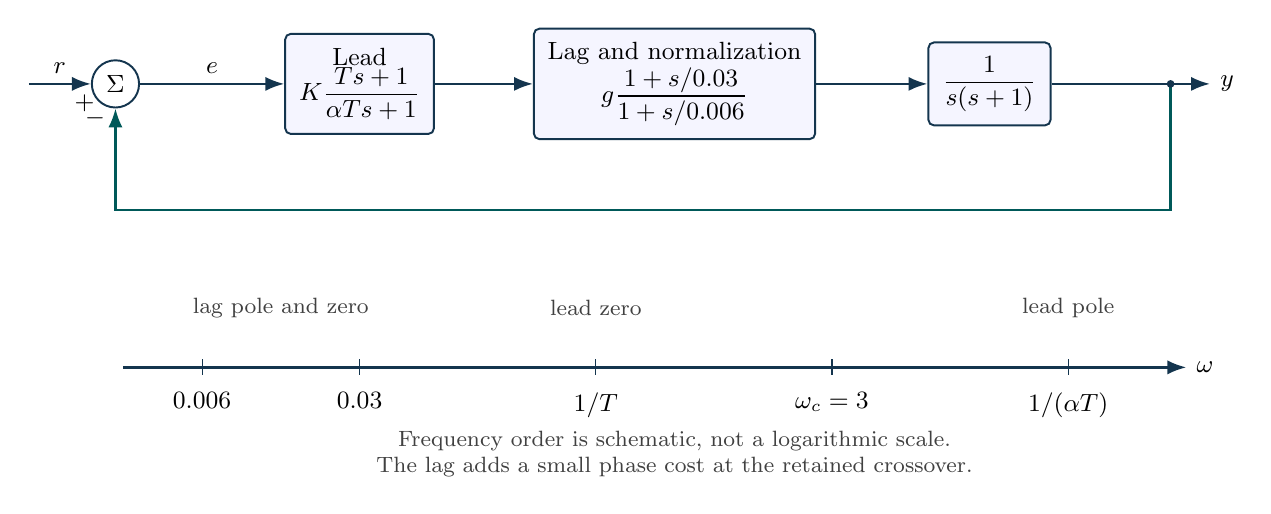
\begin{tikzpicture}[x=1cm,y=1cm,>=Latex,font=\small,
block/.style={draw=ink,fill=blue!4,rounded corners=2pt,minimum height=9mm,align=center,line width=.7pt,inner sep=5pt},
sum/.style={circle,draw=ink,fill=white,minimum size=6mm,inner sep=0pt,line width=.7pt},
sig/.style={->,draw=ink,line width=.85pt},
fb/.style={->,draw=teal!70!black,line width=.85pt},
dist/.style={->,draw=orange!75!black,line width=.85pt},
tap/.style={circle,fill=ink,inner sep=1.4pt},
note/.style={font=\footnotesize,align=center,text=black!75}]

\node[sum](e)at(.9,1.5){$\Sigma$};
\node[block](lead)at(4,1.5){Lead\\$K\dfrac{Ts+1}{\alpha Ts+1}$};
\node[block](lag)at(8,1.5){Lag and normalization\\$g\dfrac{1+s/0.03}{1+s/0.006}$};
\node[block](plant)at(12,1.5){$\dfrac{1}{s(s+1)}$};
\draw[sig](-.2,1.5)--node[above]{$r$}node[pos=.9,below]{$+$}(e);
\draw[sig](e)--node[above]{$e$}(lead);\draw[sig](lead)--(lag);\draw[sig](lag)--(plant);
\draw[sig](plant)--(14.8,1.5)node[right]{$y$};
\draw[fb](14.3,1.5)--(14.3,-.1)--(.9,-.1)--node[pos=.9,left]{$-$}(e);
\fill[ink](14.3,1.5)circle(1.4pt);
\draw[sig](1,-2.1)--(14.5,-2.1)node[right]{$\omega$};
\foreach \x/\lab in {2/0.006,4/0.03,7/{1/T},10/{\omega_c=3},13/{1/(\alpha T)}}{\draw[ink](\x,-2)--(\x,-2.2);\node[below=2mm]at(\x,-2.1){$\lab$};}
\node[note]at(3,-1.35){lag pole and zero};
\node[note]at(7,-1.35){lead zero};\node[note]at(13,-1.35){lead pole};
\node[note]at(8,-3.2){Frequency order is schematic, not a logarithmic scale.\\The lag adds a small phase cost at the retained crossover.};

\end{tikzpicture}
}
\par\small\refstepcounter{figure}\label{fig:system}\textbf{Figure \thefigure.} Lead and lag sections are drawn separately so their gain normalization and frequency ordering can be analyzed independently.\end{center}
\section{Executed computational evidence}
\VerbatimInput[fontsize=\small,breaklines=true]{results.txt}
\begin{center}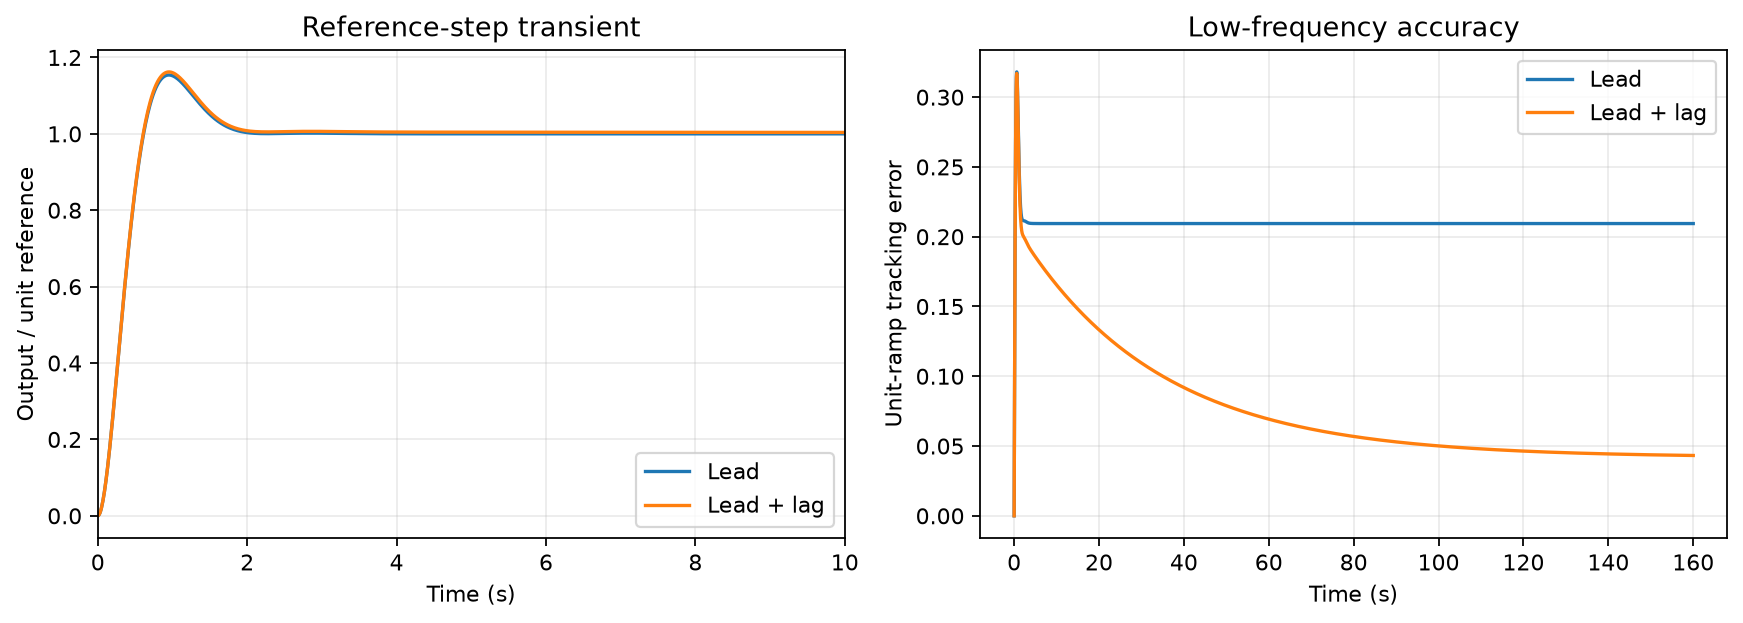
\includegraphics[width=\linewidth,height=.46\textheight,keepaspectratio]{response.png}\end{center}
\section{Method references}
The equations use standard balance laws and feedback-control methods. Further explanation: \url{https://apmonitor.com/pdc/} and \url{https://fbsbook.org/}. Implementation documentation: \url{https://python-control.readthedocs.io/en/0.10.2/}. See the repository reference catalog for individual topics and videos.
\end{document}
